\section{Work Breakdown and Schedule}
A work breakdown structure (WBS) is important to understand the complexity of the project and how components are structured. This information is particularly useful for agile development, so that releases can be scheduled based on a selection of the WBS,
 such that each component requires roughly the amount of time available in one development cycle.

\begin{figure*}[h!]
	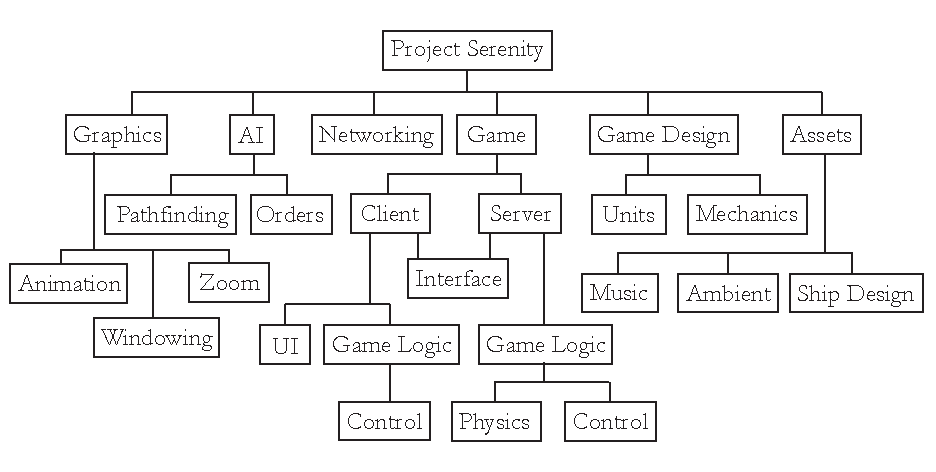
\includegraphics{res/wbs}
	\caption{Work Breakdown Structure of the game components}
\end{figure*}

From the WBS we can further break the project down into components which are suited for weekly development cycles.

\begin{table*}
	\begin{tabular}{l p{38em}}
		\toprule
		\emph{Week Number} & \emph{Release description} \\
		\midrule
		Week 3 & Project Specification Draft \\
		Week 4 & Project Specification Finished\\
		Week 5 & Networking Revision 1, Graphics Engine Revision 1, Server Game Logic\\
		Week 6 & Server Logic Revision 2, Client Logic\\
		Week 7 & Networking Revision 2, Graphics Revision 2, Ship Building Interface, Basic GUI\\
		Week 8 & Client Component, Server Component\\
		Week 9 & Game Prototype\\
		Week 10 & Progress Presentation Poster\\
		\bottomrule
		\caption{Term 1 Project schedule}
	\end{tabular}
	\label{tab:schedule}
\end{table*}

Term 2 releases will include a UI, an AI system and further improvements to the components as required. Assets such as music and additional ship designs are non-essential and will likely follow in a later release.

\begin{figure}
	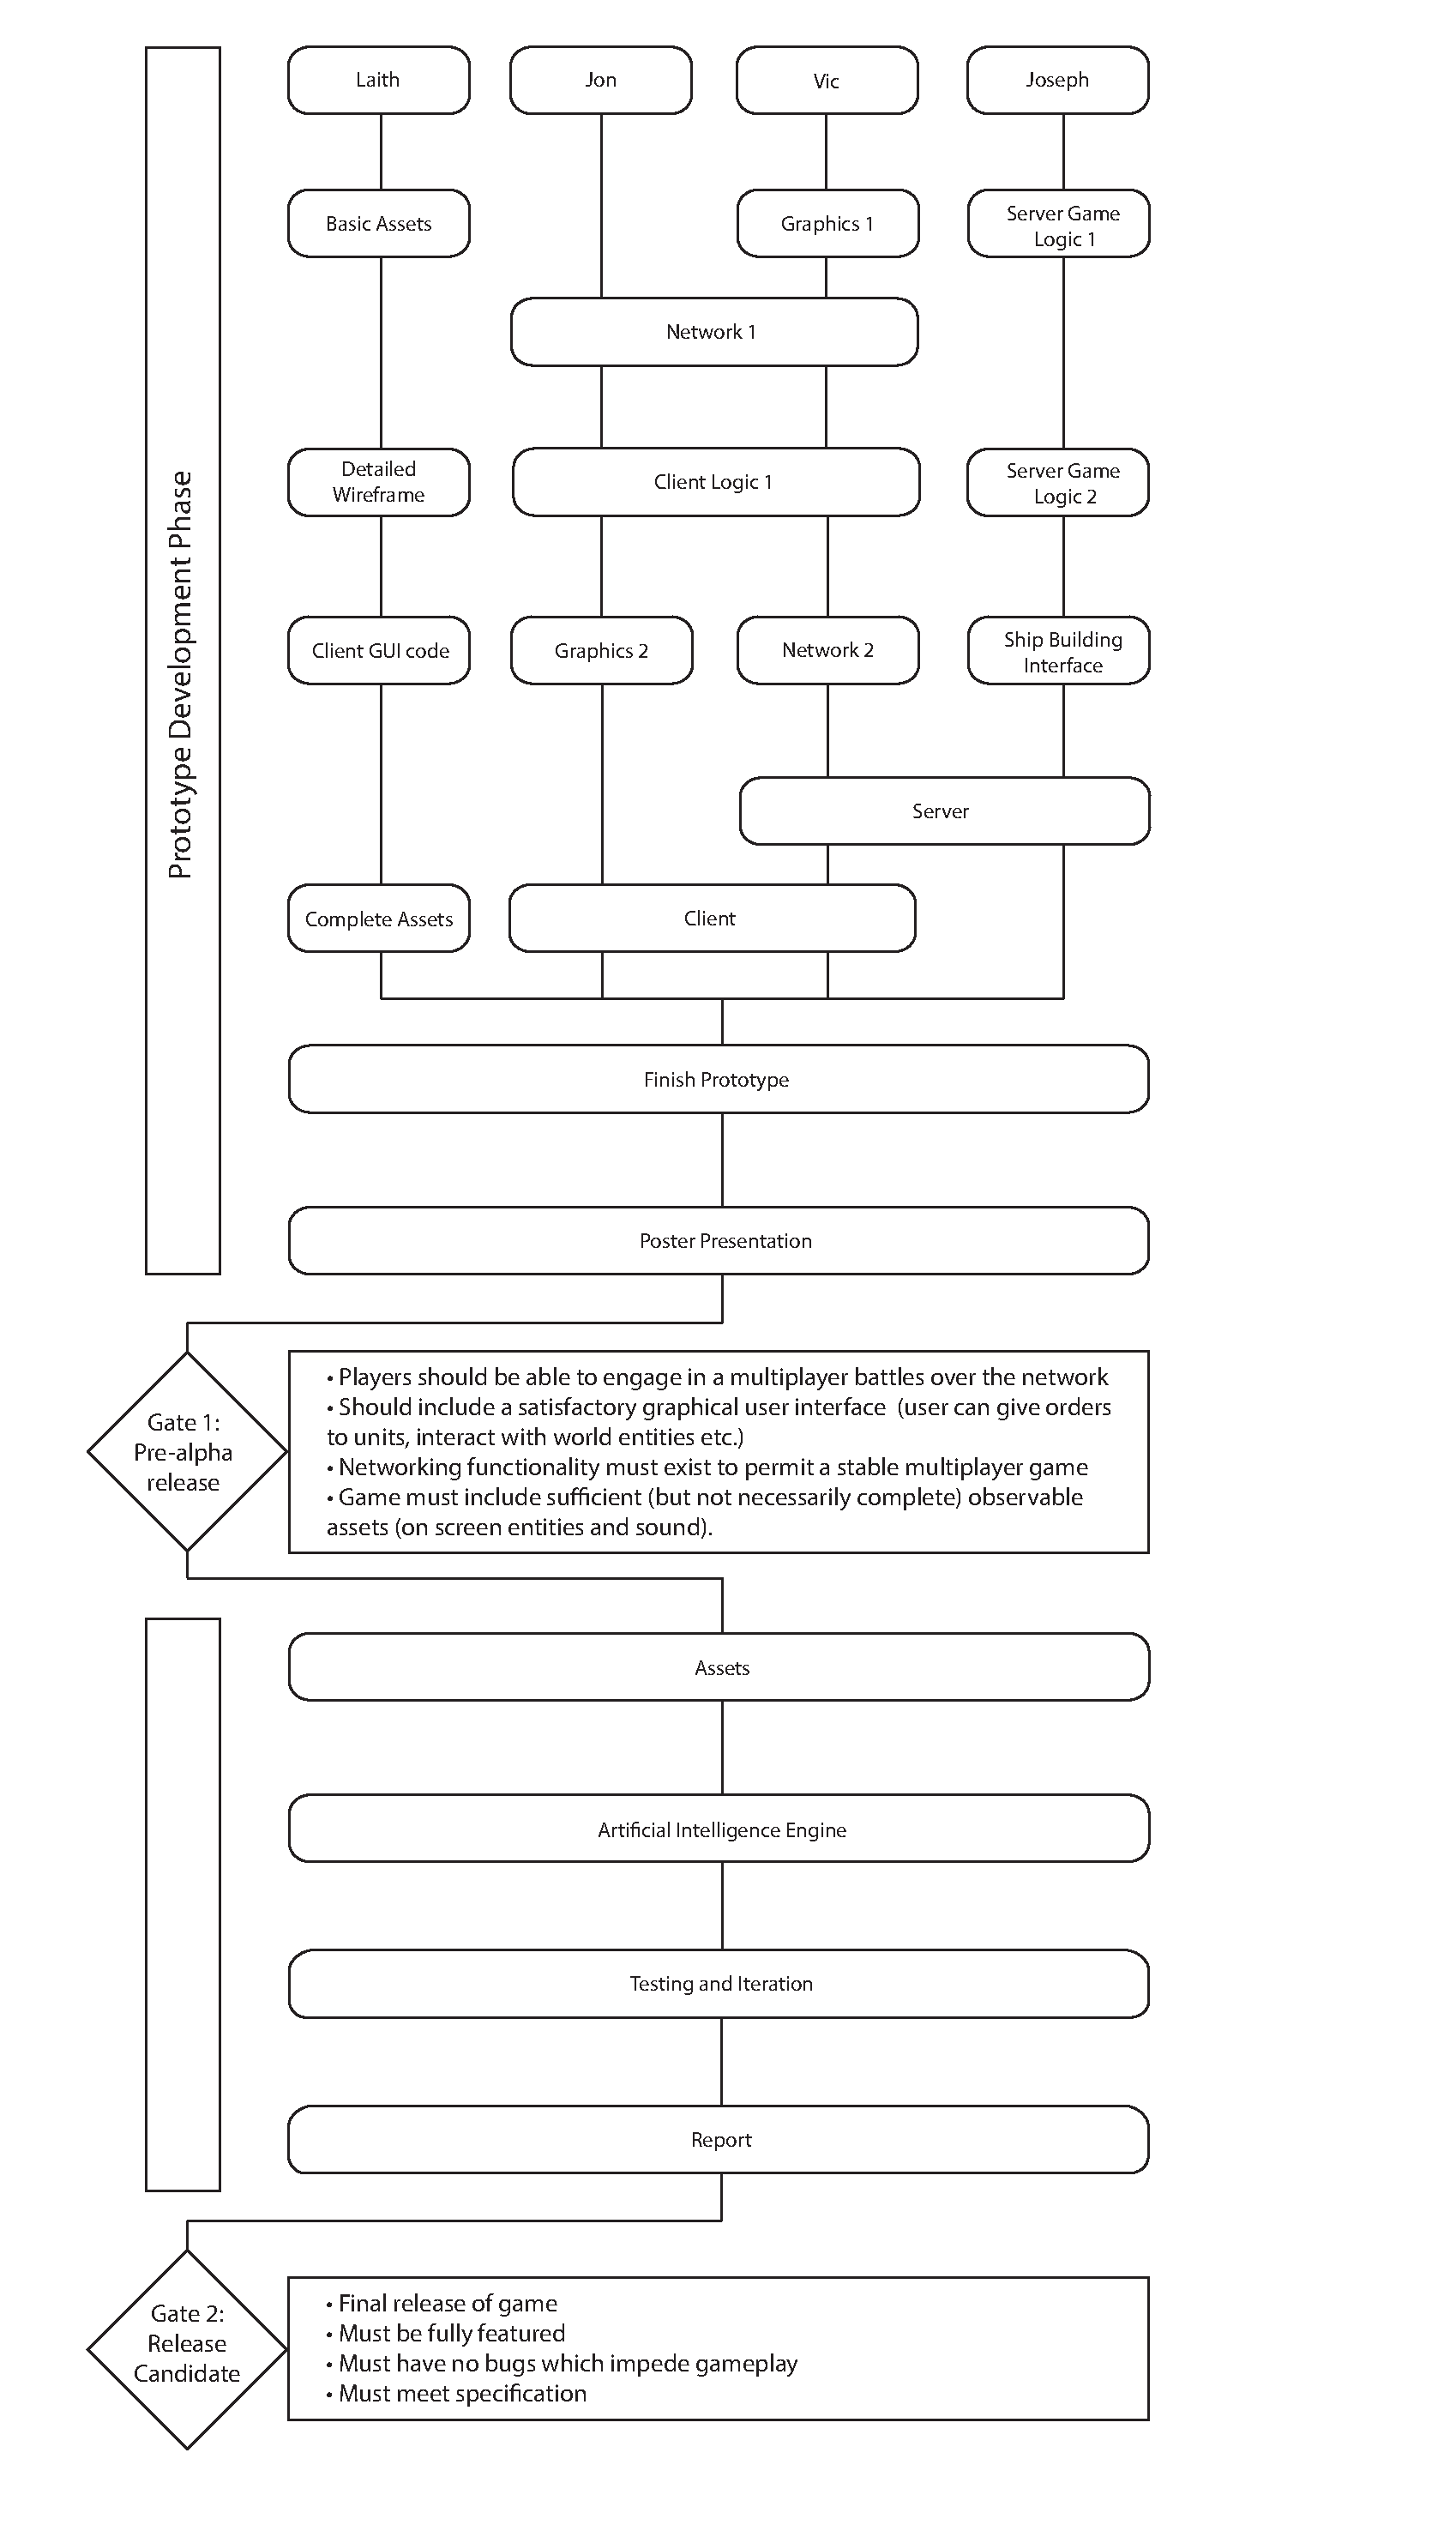
\includegraphics{res/stage_gate_diagram}
	% WE COULD PUT STANDARDS IN THE MARGIN!!! YES! CHEWING!!
	\caption{Stage-gate model of work breakdown structure}
\end{figure}